%$HeadURL: https://practicas-derive.googlecode.com/svn/trunk/funciones_elementales.tex $
%$LastChangedDate: 2008-12-08 17:44:27 +0100 (lun, 08 dic 2008) $
%$LastChangedRevision: 4 $
%$LastChangedBy: asalber $

\chapter{Funciones de varias variables:\\ Límites y continuidad}

\section*{Fundamentos Teóricos}
En muchas situaciones prácticas, el valor de una función depende
del que toman todo un conjunto de variables y no ya tan sólo de
una. El objetivo de esta práctica es el de, además de definir
dicho tipo de funciones, introducir algunos de los conceptos
básicos que se refieren a las mismas: gráfica, conjuntos de nivel,
límites y continuidad. Todo ello como extensión de las
definiciones, propiedades y conceptos ya manejados para funciones
de una única variable.

\subsection*{Función real de $n$ variables}
Una función real de varias, $n$, variables es una aplicación que
asigna a cada punto $\vec{x}$ de un conjunto $A$ contenido en
$\mathbb{R}^n$, $ \vec x  = \left( {x_1 ,x_2 ,...,x_n } \right)$,
un único número real $f\left( {\vec x } \right) = f\left( {x_1
,x_2 ,...,x_n } \right)$


\[
f:\begin{array}{*{20}c}
   {A \subset \mathbb{R}^n  \to \mathbb{R}}  \\
   {\vec x  \to f\left( {\vec x } \right)}  \\

 \end{array}
\]

El conjunto $A$ se llama \emph{Dominio} de la función y los
valores de $f$ constituyen el \emph{Rango o Recorrido}.

De $f$ se dice que es una \emph{Función Real de Variable
Vectorial}, y también que se trata de un \emph{Campo Escalar}.
Esto último sobre todo en problemas de Física, en los que abundan
ejemplos de este tipo de funciones: la temperatura como función de
las coordenadas del punto, $T(x,y,z)$; la presión en el seno de un
fluido con idénticas variables, $P(x,y,z)$; o el potencial
eléctrico también como $V(x,y,z)$, entre otros.

\subsection*{Gráfica de una función real de $n$ variables}

Recordemos que la gráfica de una función de una única variable,
$f: A \subset \mathbb{R}  \to \mathbb{R}$, es un subconjunto de
$\mathbb{R}^2$ que consta de todos los puntos $(x,f(x))$. De igual
forma se define la \emph{Gráfica de una Función Real de Variable
Vectorial}, $f: A \subset \mathbb{R}^n  \to \mathbb{R}$, como el
subconjunto de $\mathbb{R}^{n+1}$ que consta de todos los puntos $
\left( {\vec x ,f\left( {\vec x } \right)} \right)$.

\begin{figure}[h!]
\begin{center}
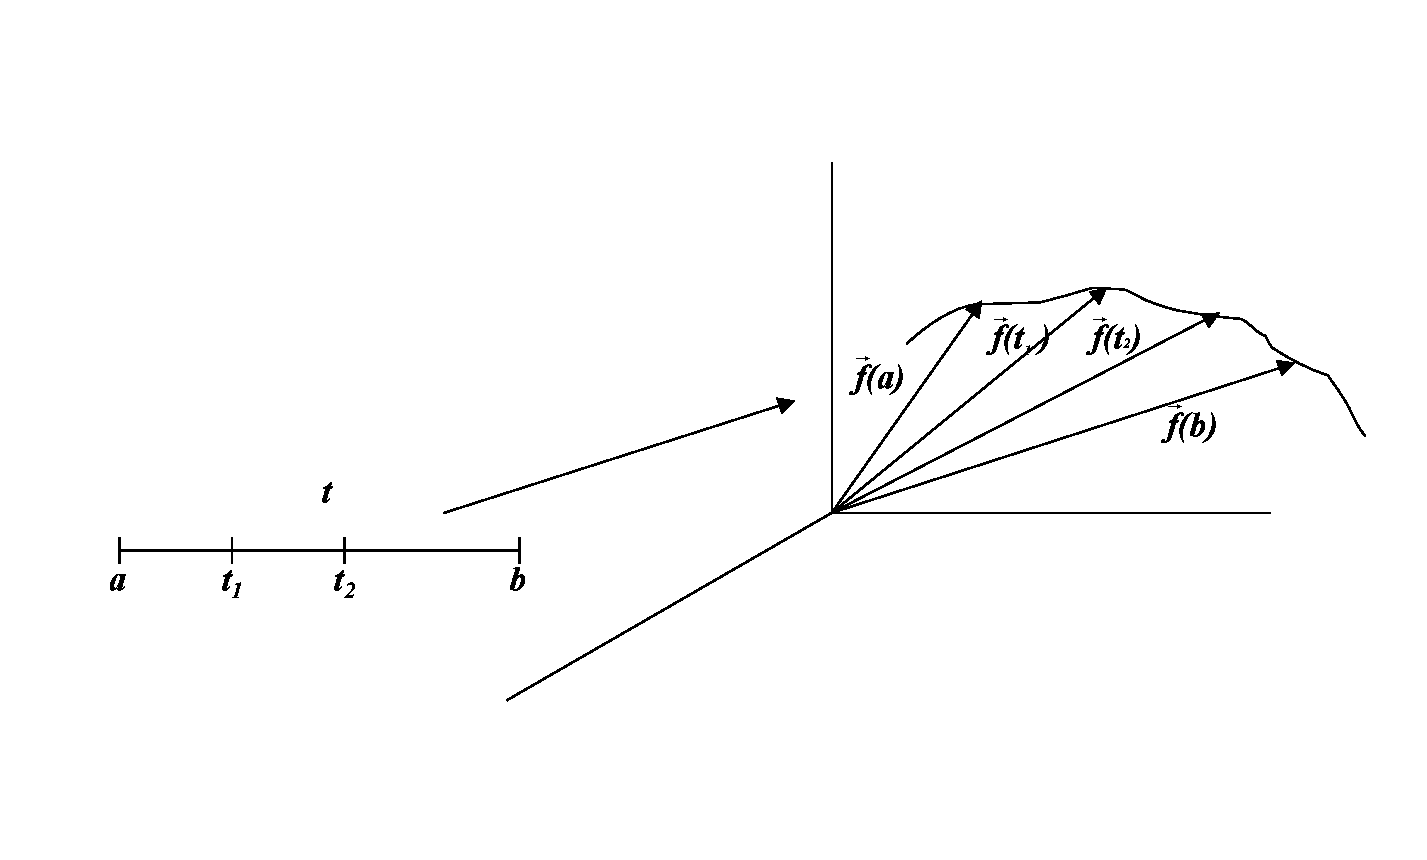
\includegraphics[scale=0.4]{img/limites_varias_variables/grafica}
\caption{Gráfica de una función de dos variables}
\end{center}
\end{figure}


Por ejemplo, si $f$ es una función de dos variables, $f(x,y)$, la
gráfica de $f$ es una superficie en $\mathbb{R}^3$ compuesta por
los puntos $(x,y,f(x,y))$, o de otra forma $(x,y,z)$, donde
$z=f(x,y)$. Además, cualquiera de los programas de Cálculo para
ordenador ofrecen ya la posibilidad de representar las gráficas
``tridimensionales" de funciones de dos variables, proyectadas en
el plano de la pantalla. Para funciones de tres o más variables no
hay un reflejo gráfico para la gráfica de una función, ya que
necesitaríamos cuatro o más coordenadas.




\subsection*{Conjunto de nivel de una función real de $n$
variables}

Sea $f: A \subset \mathbb{R}^n  \to \mathbb{R}$ una función real
de varias variables, y sea $c \in \mathbb{R}$ una constante.
Definimos el \emph{Conjunto de Nivel de Valor $c$} como aquellos
puntos $\vec x  \in A$ para los cuales $f\left( {\vec x } \right)
= c$.

En el caso de las funciones de dos variables, $f(x,y)$, el
conjunto de nivel recibe el nombre de curva de nivel. Por lo
tanto, la Curva de Nivel $c$ de la superficie $z=f(x,y)$ es el
conjunto formado por los puntos del plano $(x,y)$ pertenecientes
al dominio de $f$ tales que  $f(x,y)=c$.

El ejemplo más frecuente de curvas de nivel aparece en los mapas
topográficos. Si consideramos que $z=f(x,y)$ es la altura sobre el
nivel de mar del punto de coordenadas $(x,y)$, y unimos en el
plano los puntos de igual altura, obtenemos unas curvas que
permiten observar la situación de montañas y valles. Otro ejemplo
de curvas de nivel lo encontramos en los mapas con las
predicciones del tiempo, que presentan las isobaras que surgen al
unir en el plano los puntos de igual presión.

\begin{figure}[h!]
\begin{center}
\includegraphics[scale=0.4]{img/limites_varias_variables/conjuntonivel}
\caption{Conjunto de nivel de una función de dos variables}
\end{center}
\end{figure}


\subsection*{Límite de una función real de $n$ variables}

Sea $f: A \subset \mathbb{R}^n  \to \mathbb{R}$ y un punto $\vec
a$ de $\mathbb R^n$, que no tiene necesariamente que pertenecer al
dominio de $f$ con tal de que sea punto de acumulación del mismo
(es decir, sí que deben existir puntos de $A$ tan próximos como se
quiera a $\vec a$). Entonces, de forma similar a lo que sucedía
con las funciones de una única variable, y de manera informal,
decimos que:

\[
\mathop {\lim }\limits_{\vec x \to \vec a} f\left( {\vec x}
\right)=l
\]
si $f\left( {\vec x} \right)$ se aproxima cada vez más a $l$ a
medida que $\vec x$ se aproxima a $\vec a$.

No obstante, en $\mathbb R^n$ el concepto de tendencia o
aproximación es mucho más complejo que en $\mathbb R$, ya que para
un cierto $a \in \mathbb R$ tan sólo se puede tender al mismo
desde valores mayores, y hablaríamos de límite por la derecha, o
desde valores menores, y hablaríamos de límite por la izquierda;
mientras que, por ejemplo, en $\mathbb R^2$ podríamos aproximarnos
al punto $\vec a$ de coordenadas $(x_0,y_0)$ a través de infinitas
rectas diferentes, e incluso a través de infinitas curvas
(parábolas, exponenciales, ...); e igual sucedería en cualquier
otro $\mathbb R^n$.

Lo anterior da lugar al siguiente importante teorema, de contenido
similar al que en $\mathbb R$ afirma que el límite existe si
existen los límites laterales y coinciden:


\begin{teorema}
Si existe el límite de $f: A \subset \mathbb{R}^n  \to \mathbb{R}$
en el punto $\vec a$ y vale $l$, entonces existe el límite sea
cual fuere la forma de tender hacia $\vec a$ y vale $l$.
\end{teorema}

Lo anterior puede utilizarse para demostrar la no existencia del
límite, sin más que considerar dos tendencias diferentes y ver que
los límites que se obtienen no son iguales. Sin embargo, no puede
utilizarse para demostrar la existencia del mismo, ya que habría
que considerar las infinitas tendencias diferentes. Por ello, el
cálculo de límites de funciones de dos o más variables resulta
complejo y difícil de plasmar en un algoritmo, lo cual se traduce
en que los programas actuales de Cálculo con ordenador realizan
correctamente tan sólo algunos de los límites de funciones de este
tipo.

Mucho más fácil que el cálculo del límite de una función de varias
variables, resulta el cálculo de los denominados \emph{Límites
Iterados}, también llamados \emph{Reiterados o Sucesivos}, que
definimos a continuación:

Sea $f: A \subset \mathbb{R}^n  \to \mathbb{R}$, $\vec x \in A$ un
punto del dominio de coordenadas $\left(x_1,x_2,...,x_n\right)$, y
$\vec a=\left(a_1,a_2,...,a_n\right)$ el punto al que tendemos. Se
definen los límites iterados si existe:

\[
\mathop {\lim }\limits_{x_1  \to a_1 } \left( {\mathop {\lim
}\limits_{x_2  \to a_2 } \left( {...\left( {\mathop {\lim
}\limits_{x_n  \to a_n } f\left( {\vec x} \right)} \right)}
\right)} \right)
\]
y todas las reordenaciones de los diferentes límites.

Por ejemplo, en $\mathbb R^2$: $\vec x=(x,y)$, $\vec a=(x_0,y_0)$;
y resultan dos posibles límites iterados:


\[
\mathop {\lim }\limits_{x \to x_0 } \left( {\mathop {\lim
}\limits_{y \to y_0 } f(x,y)} \right)
\]

\[
\mathop {\lim }\limits_{y \to y_0 } \left( {\mathop {\lim
}\limits_{x \to x_0 } f(x,y)} \right)
\]

De nuevo, podría demostrarse que si existe $ \mathop {\lim
}\limits_{\vec x \to \vec a} f\left( {\vec x} \right)$ y los
límites reiterados de $f$, entonces todos coinciden. Lo cual nos
permite asegurar que si los límites reiterados de una función en
un punto $\vec x =\vec a$ existen y son diferentes, entonces no
existe $ \mathop {\lim }\limits_{\vec x \to \vec a} f\left( {\vec
x} \right)$.

\subsection*{Continuidad de una función real de $n$ variables}

De manera similar a lo que secede con las funciones de una única
variable, $f: A \subset \mathbb{R}^n  \to \mathbb{R}$ se dice que
es \emph{Continua en el Punto} $\vec a \in A$ si se verifican:

\begin{itemize}
  \item Existe $f\left(\vec a\right)$.
  \item Existe $\mathop {\lim }\limits_{\vec x \to \vec a} f\left( {\vec x}
\right)=l$.

\item Ambos coinciden: $f\left(\vec a\right)=l$.
\end{itemize}

Y diríamos que $f$ es continua en todo un subconjunto de su
dominio si es continua en todos los puntos del mismo.

Si tenemos una función de dos variables, $f(x,y)$, la continuidad
en un conjunto significaría geométricamente que la superficie
$z=f(x,y)$ no tiene saltos ni agujeros en todo el conjunto.





\section{Ejercicios resueltos}

\begin{enumerate}[leftmargin=*]
\item Dada la función:

\[
f(x,y) = \frac{1} {{x^2  + 2y^2  + 1}}
\]

\begin{enumerate}
  \item Definirla y representar su gráfica. Una vez representada,
  rotarla, agrandarla, contraerla, hacer zoom hacia fuera y hacia
  dentro para cambiar la escala de representación, y cambiar el
  número de paneles para representar la gráfica con una trama más
  o menos tupida.

\begin{indicacion}
{

\begin{enumerate}

\item Para definirla, utilizar el operador definición $:=$, y para
representarla, utilizar el botón \boton{Ventana 3D}, y una vez en el
entorno tridimensional, utilizar el botón \boton{Representar}.

\item

\begin{itemize}

\item Para rotarla, utilizar los botones \boton{Rota la gráfica},
\boton{Girar hacia la izquierda}, \boton{Girar hacia la derecha},
\boton{Rotar hacia arriba} y \boton{Rotar hacia abajo}.

\item Para agrandarla y contraerla utilizar los botones
\boton{Magnificar} y \boton{Contraer}. Observar cómo, tanto al
agrandar como al contraer, no cambiamos la escala del cubo en el que
se muestra la gráfica, y por tanto seguimos viendo la misma porción
de gráfica alejada o acercada.

\item Un efecto similar al que se genera mediante la rotación de
la gráfica, combinada con un acercamiento o alejamiento, lo podemos
obtener mediante el botón \boton{Fijar la posición del ojo}.

\item Para hacer zoom hacia fuera o hacia dentro utilizar los
botones \boton{Zoom hacia fuera} y \boton{Zoom hacia dentro}.
Comprobar cómo varía la escala del cubo en el que se muestra la
gráfica al hacer zoom. En definitiva, cambiamos la porción de
gráfica que vemos, pero no la posición desde la que la miramos. Un
efecto similar se obtiene con los botones \boton{Ajuste del
mínimo/máximo} y \boton{Restablece rango}.

\item Para cambiar el entramado de la gráfica, lo más cómodo es
utilizar el menú contextual que aparece al pulsar el botón derecho
del ratón sobre la gráfica y utilizar \menu{Editar->Parámetros de la
gráfica->Número de Paneles}.
\end{itemize}

\end{enumerate}

}
\end{indicacion}

  \item Representar la curva de nivel que se obtiene para
  $f(x,y)=1/2$.

\begin{indicacion}
{Igualar la definición de la función a 1/2 y representar mediante el
botón \boton{Ventana 2D}. Recordar que las curvas de nivel son
puntos del plano $XY$ en los que la función toma el mismo valor (la
gráfica tridimensional presentaría igual altura).

}
\end{indicacion}


  \item Utilizar la función \comando{VECTOR(u,k,m,n)} para dibujar todas las
  curvas de nivel de la forma $f(x,y) = 1/k$, donde $k$ toma los
  valores naturales de $2$ a $10$ (tener en cuenta que, en la función \comando{Vector},
  $u$ sería la expresión de las curvas de nivel $f(x,y) = 1/k$, y
$k$ un índice de variación que toma valores entre $m$ y $n$).

\begin{indicacion}
{

\begin{enumerate}

\item La función \comando{VECTOR} de Derive, genera un
vector cuyas componentes son la función $u$, que depende de un
índice $k$, variando el mismo entre los valores $m$ y $n$. En
nuestro caso, si introducimos en Derive el comando:

\begin{center}
\comando{VECTOR}$(f(x,y)=1/k,k,2,10)$
\end{center}

se genera un vector cuyas 9 componentes son:
\[
[f(x,y)=1/2,f(x,y)=1/3,...,f(x,y)=1/10]
\]

\item Para representar a la vez todas esas curvas de nivel
generadas, simplemente marcamos la expresión que las contiene, y
procedemos a representar en la \boton{Ventana 2D} de igual forma que
representaríamos cualquier función de una única variable.
\end{enumerate}

}
\end{indicacion}

\end{enumerate}

\item Dada la función:


\[
f(x,y) = \frac{{xy}} {{x^2  + 3y^2 }}
\]

\begin{enumerate}
  \item Definirla y representar su gráfica. Observar
  la gráfica desde diferentes perspectivas,
  con especial interés por lo que ocurre en las
  cercanías del punto (0,0).

\begin{indicacion}
{Para definirla, utilizar el operador de definición :=, y para
cambiar la perspectiva con el objetivo de observar lo que ocurre en
las cercanías del punto (0,0), utilizar los botones
\boton{Magnificar} y los de \boton{Rotación} (hacia arriba y hacia
abajo) y de \boton{Giro} (a izquierda y derecha), además de cambiar
el número de paneles que se muestran por defecto, con el menú
contextual (botón derecho del ratón) y \menu{Editar->Parámetros de
la Gráfica->Número de paneles}.

}
\end{indicacion}

  \item ¿Se puede calcular el valor de la función en el punto
  (0,0)? ¿Puede la función ser continua en (0,0)?.

\begin{indicacion}
{

\begin{enumerate}

\item Para ver cuál es el valor de la función en el punto $(0,0)$,
intentar obtener $f(0,0)$.

\item Para responder a la pregunta sobre si la función puede ser
continua en $(0,0)$, simplemente considerar que la función no está
definida en dicho punto, con lo cual, difícilmente puede ser
continua.

\end{enumerate}

}
\end{indicacion}


  \item Calcular los límites iterados en $(0,0)$. A la vista de
  dichos límites, ¿qué concluimos sobre la existencia, si es que existe, y el valor
  de $\mathop {\lim }\limits_{\left( {x,y} \right) \to \left( {0,0}
  \right)} f\left( {x,y} \right)$?

\begin{indicacion}
{




\begin{enumerate}

\item Para calcular los límites iterados, tomar el límite (botón
\boton{Calcular un límite}) de la función inicialmente considerando
como variable $x$, y luego proceder a calcular el límite del límite
anterior pero ahora tomando como variable $y$:

\[
\mathop {\lim }\limits_{y \to 0 } \left( {\mathop {\lim
}\limits_{x \to 0 } f(x,y)} \right)
\]

Repetir el mismo proceso pero intercambiando las variables, es
decir, inicialmente el límite con respecto a $y$ y luego con
respecto a $x$:

\[ \mathop {\lim }\limits_{x \to 0 } \left( {\mathop {\lim
}\limits_{y \to 0 } f(x,y)} \right)
\]

\item Sobre la existencia del límite de la función, recordar que
para que el límite exista los iterados deben existir y coincidir,
pero se trata de una condición necesaria aunque no suficiente. Por
lo tanto, si los límites iterados no existen, o si existen pero
son diferentes, concluimos que no existe el límite; pero si
existen y son iguales, no podemos concluir que el límite exista.

\end{enumerate}

}
\end{indicacion}


  \item Calcular sus límites direccionales en el mismo punto a través de la familia
  de rectas $y=mx$. A la vista de los resultados, ¿qué concluimos
  sobre la posible existencia del límite en dicho punto?.

\begin{indicacion}
{Para calcular los límites direccionales a través de la familia de
rectas $y=mx$:

\begin{enumerate}

\item En la definición de la función sustituir $y$ por $mx$.

\item Calcular el límite cuando $x$ tiende a 0 de la expresión
resultante (botón \boton{Calcular un límite}). Observar que la
función resultante no depende de $x$ y, por lo tanto, el programa no
propone $x$ como variable en la que calcular el límite (tan sólo
propone $m$). No obstante, podemos poner $x$ en el cuadro de diálogo
mediante el teclado.

\item Como el límite final resultante depende de $m$ quiere ello
decir que el valor del límite depende de la pendiente de la recta
$y=mx$, es decir, es diferente según diferentes tendencias hacia
el punto, lo cual implica que no existe el límite.

\end{enumerate}

}
\end{indicacion}


\end{enumerate}

\item Dada la función:

\[
f(x,y) = \left\{ {\begin{array}{*{20}c}
   0 & {\text{si}} & {x <0}  \\
   \cos{(x^2+y^2)}& {\text{si}} & {x\geq 0}  \\

 \end{array} } \right.
\]

\begin{enumerate}
  \item Utilizar la función condicional de Derive $\comando{If(condicion,opcion 1,opcion 2)}$,
   para definir la función $f(x,y)$.


\begin{indicacion}
{Para la función $f(x)$, podemos, para su definición, utilizar la
función condicional de Derive \comando{If(condición,opción 1,opción
2)}, de tal forma que si se cumple la \comando{condición} el
programa realizará la \comando{opción 1}, y si no se cumple
realizará la \comando{opción 2}. La función condicional de Derive,
\comando{If}, entre otras muchas posibilidades sirve para introducir
funciones definidas a trozos. En nuestro caso la \comando{condición}
es $x<0$, la \comando{opción 1} es $0$, y la \comando{opción 2} es
$\cos(x^2+y^2)$.

Así, la función $f(x,y)$ puede definirse mediante:

\[
f(x,y):=\comando{IF}(x<0,0,\cos(x^2+y^2))
\]

}
\end{indicacion}


  \item Representar su gráfica. A la vista de la gráfica, ¿crees
  que la función será continua en $x=0$?.


\begin{indicacion}
{Para representar la gráfica, botón \boton{Ventana 3D}, y una vez en
el entorno de dibujo de funciones de dos variables, botón
\boton{Representar}. Convendrá editar la gráfica (botón derecho del
ratón sobre la gráfica y menú \menu{Editar}) y aumentar el número de
paneles. }
\end{indicacion}


  \item Demostrar que la función no es continua en $(x,y)=(0,0)$.

\begin{indicacion}
{Se puede demostrar tomando límites en el punto $(0,0)$ a través
de rectas de la forma $y=mx$. Por ejemplo se puede tomar la recta
$y=0$ y ver qué sucede cuando $x$ tiende a cero por la derecha
(por los mayores que 0), o por la izquierda (por los menores que
0).


}
\end{indicacion}


\end{enumerate}
\end{enumerate}


\section{Ejercicios propuestos}
\begin{enumerate}

\item Para la función:

\[
f(x,y) = 10 - \sqrt {x^2  + y^2 }
\]

\begin{enumerate}
\item Representar su gráfica. A la vista de la gráfica, ¿qué forma
tendrán sus curvas de nivel?.

\item Representar sus curvas de nivel para la $f(x,y)=k$, donde
$k$ toma los valores naturales desde 1 hasta 5.
\end{enumerate}

\item Demostrar que no existe el límite:

\[
\mathop {\lim }\limits_{\left( {x,y} \right) \to \left( {0,0}
\right)} \frac{{\left( {x - y} \right)^2 }} {{x^2  + y^2 }}
\]

\item Sea la función:

\[
f(x,y) = \left\{ {\begin{array}{*{20}c}
   {\dfrac{{x^2 }}
{{x^2  + y^2 }}} & {\text{si}} & {\left( {x,y} \right) \ne \left( {0,0} \right)}  \\
   0 & {\text{si}} & {\left( {x,y} \right) = \left( {0,0} \right)}  \\

 \end{array} } \right.
\]

Estudiar su continuidad en todo $\mathbb{R}^2$ (para definirla,
utilizar la función condicional \comando{If}, y para introducir la
\comando{condición} $(x,y)=(0,0)$ utilizar $x=0$ \comando{and}
$y=0$).
\end{enumerate}